\chapter{Hardware Details}\label{app:hard_appendix}

\section{Additional technical information on Game Towers}

\begin{figure}[h]
    \centering
    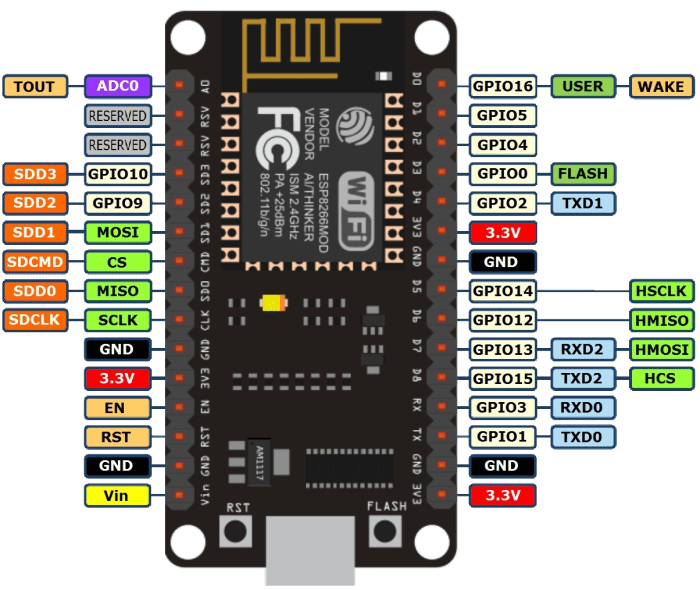
\includegraphics[draft=false, width=5cm]{images/03-foundation/node_mcu_pinout}
  \caption{The pinout of the NodeMCU V3 ESP8266 ESP-12E WiFi module used for data transmission.}
  \label{fig:tower_board}
\end{figure}

\begin{figure}[H]
	\centering
	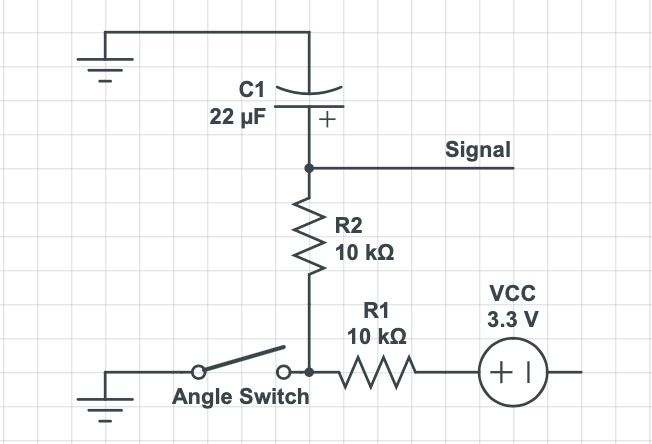
\includegraphics[draft=false, width=5cm]{images/03-foundation/tilt_sensor_circuit}
	\caption{The circuit for detecting when a tower has fallen. A tilt switch detects the inclination and the low-pass filter smooths out noise from vibrations such as those caused by the player touching the tower. The signal wire is attached to a pin on the NodeMCU V3 ESP8266 ESP-12E WiFi Module, which allows communication with the robot's onboard computer.}
    \label{fig:tilt_circuit} 
\end{figure}

\section{Kinematics of a 3-wheeled omni-directional robot}
The pose of a rigid mobile robot is commonly described by six variables, its three-dimensional Cartesian coordinates and its three Euler angles (roll, pitch, yaw) relative to an external coordinate frame~\citep{thrun_probabilistic_2005}. If the robot is considered as moving on a planar surface, this reduces to two Cartesian coordinates and an orientation angle.
The kinematic model of an omni-directional base consists of an equation of motion of the robot in function of wheels velocity without considering the forces acting on the system. In this section, a kinematic model for a 3-wheeled omni-directional robot will be derived.

\begin{figure}[H]
  \centering
  \begin{subfigure}[b]{0.4\textwidth}
     \centering
      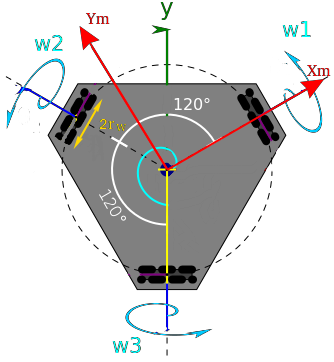
\includegraphics[draft=false,width=4cm, height=3.5cm]{images/03-foundation/triskarbase1}
	\caption{}
	\label{triskar1} 
  \end{subfigure}
  \begin{subfigure}[b]{0.4\textwidth}
  \centering
      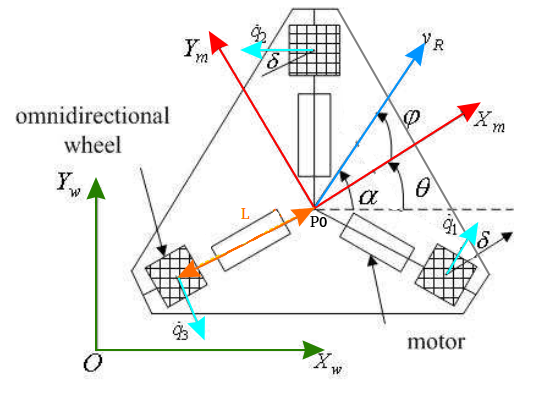
\includegraphics[draft=false,width=4cm, height=3.5cm]{images/03-foundation/triskarbase2}
	\caption{}
	\label{triskar2} 
  \end{subfigure}
  \caption{Kinematics diagram of the base of an omnidirectional robot. a) omni-directional base wheels displacement angle. b) omni-directional base reference frames and velocities.}
\end{figure}

Considering the figure (\ref{triskar2}), each wheel of the robot is driven by a DC motor and its center has the same distance L to the robot center of mass $P_0$. we define the fixed world coordinate system [$X_R$, $Y_R$] and a mobile robot fixed frame [${x}^m_R$, ${y}^m_R$] that is parallel to the floor and whose origin locates at $P_0$.\\
The robot's orientation is denoted by angle $\theta$, which is the direction angle of the axis $X_m$ in the world coordinate system (positive in the
counterclockwise direction) and $\delta$ refers to the wheel orientation in the robot coordinate system and it is equal to 30 degrees in our considered example.
\\
$\alpha$ and $\phi$ denote the direction of the robot translation velocity $v_R$ observed in the world and robot coordinate systems, respectively.\\
We consider \textbf{v} = [$\dot{x}^m_R,\dot{y}^m_R,\omega$]$^T$ the robot velocities observed in the robot coordinate system; \\
$\mathbf{\dot{q}}$ = [$\dot{q}_1,\dot{q}_2,\dot{q}_3$]$^T$ is the vector of wheel velocities equal to the i-th wheel radius $r_\omega$ multiplied by the wheel angular velocity.

We introduce the transformation matrix from the robot coordinate system to the world coordinate system:
\begin{equation}
^wR_m(\theta)=\begin{bmatrix}
\cos(\theta) &-\sin(\theta)\\
\sin(\theta) & \cos(\theta)\\
\end{bmatrix}
\end{equation}

We can transform from robot to world coordinates system as:
\begin{equation}
\begin{bmatrix}
\dot{x}_R\\
\dot{y}_R\\
\dot{\theta}
\end{bmatrix} =
\begin{bmatrix}
\cos(\theta) &-\sin(\theta) & 0\\
\sin(\theta) & \cos(\theta) & 0\\
0 & 0 & 1
\end{bmatrix}
\begin{bmatrix}
\dot{x}^m_R\\
\dot{y}^m_R\\
\omega
\end{bmatrix}
\label{rotation}
\end{equation}

$P_0$ denotes the position of the center of mass with respect to the world frame as:
\begin{equation}
P_0 = 	\begin{bmatrix}
x_R\\
y_R\\
\end{bmatrix}
\end{equation}

The position $[x_i\quad y_i]^T$ of each wheel can be given with respect to the center of mass of the robot, for i=1,2,3:
\begin{equation}
P_i = 	\begin{bmatrix}
x_{Ri}\\
y_{Ri}\\
\end{bmatrix} = 
^wR_m(\theta)\cdot L
\begin{bmatrix}
1\\
0\\
\end{bmatrix}
\end{equation}

Again, considering that the wheels present a displacement of $120^\circ$ between each other we can deduce the following three vectors:

\begin{equation}
\begin{cases} 
P_1 = 	
^wR_m(0)\cdot L
\begin{bmatrix}
1\\
0\\
\end{bmatrix} =
L
\begin{bmatrix}
1\\
0\\
\end{bmatrix}
\\ 
P_2 = 	
^wR_m(\frac{2\pi}{3})\cdot L
\begin{bmatrix}
1\\
0\\
\end{bmatrix} =
\cfrac{L}{2}
\begin{bmatrix}
-1\\
\sqrt{3}\\
\end{bmatrix}
\\ 
P_3 = 	
^wR_m(\frac{4\pi}{3})\cdot L
\begin{bmatrix}
1\\
0\\
\end{bmatrix} =
-\cfrac{L}{2}
\begin{bmatrix}
-1\\
\sqrt{3}\\
\end{bmatrix}
\\ 
\end{cases} 
\end{equation}

We now define the normal unit vectors of each wheel, representing the translational direction, as follows:
\begin{equation}
D_i =  \frac{1}{L}R(\frac{\pi}{2})P_i\qquad i=1,2,3 \\
\end{equation}
\begin{equation}
\begin{cases}
D_1 = \begin{bmatrix}0 \\ 1 \end{bmatrix} \\
D_2 = -\cfrac{1}{2}\begin{bmatrix}\sqrt{3} \\ 1 \end{bmatrix} \\
D_3 = \cfrac{1}{2}\begin{bmatrix}\sqrt{3} \\ -1 \end{bmatrix} \\
\end{cases}
\end{equation}

Then the translational velocity $q_i$ as depicted in figure~\ref{triskar2} can be written in the robot reference frame as follows:
\begin{equation}
\begin{cases}
\dot{q_1} =\cos(\delta)\dot{x^m _R}+\sin(\delta)\dot{y^m _R}+L{\omega}\\
\dot{q_2} =-\cos(\delta)\dot{x^m _R}+\sin(\delta)\dot{y^m _R}+L{\omega}\\
\dot{q_3} =-\dot{y^m _R}+L{\omega}\\
\end{cases}
\end{equation}

The kinematic model with respect to the robot coordinate system is given by:
\begin{equation}
\begin{bmatrix}
\dot{x}^m _R\\
\dot{y}^m _R\\
{\omega}
\end{bmatrix} =
\begin{bmatrix}
\cos(\delta) & \sin(\delta) & L\\
-\cos(\delta) & \sin(\delta) & L\\
0 & -1 & L
\end{bmatrix}^{-1}
\begin{bmatrix}
\dot{q_1}\\
\dot{q_2}\\
\dot{q_3}\\
\end{bmatrix}	
\label{model1}
\end{equation}
\begin{equation*}
	\begin{bmatrix}
		\dot{x}^m _R\\
		\dot{y}^m _R\\
		{\omega}
	\end{bmatrix} =
	\begin{bmatrix}
		\frac{\sqrt{3}}{3} & -\frac{\sqrt{3}}{3} & 0\\
		\frac{1}{3} & \frac{1}{3} & -\frac{2}{3}\\
		\frac{1}{3L} & \frac{1}{3L} & \frac{1}{3L}
	\end{bmatrix}
	\begin{bmatrix}
		\dot{q_1}\\
		\dot{q_2}\\
		\dot{q_3}\\
	\end{bmatrix}	
\end{equation*}

If we now consider the equation~\ref{rotation} the kinematic model with respect to the world coordinate system is described as:
\begin{equation}
\begin{bmatrix}
\dot{x}_R\\
\dot{y}_R\\
\dot{\theta}
\end{bmatrix} =
\begin{bmatrix}
\frac{2}{3}\cos(\theta+\delta) & -\frac{2}{3}\cos(\theta-\delta) & \frac{2}{3}\sin(\theta)\\
\frac{2}{3}\sin(\theta+\delta) & -\frac{2}{3}\sin(\theta-\delta) & \frac{2}{3}\cos(\theta)\\
\frac{1}{3L} & \frac{1}{3L} & \frac{1}{3L}
\end{bmatrix}
\begin{bmatrix}
\dot{q_1}\\
\dot{q_2}\\
\dot{q_3}\\
\end{bmatrix}	
\label{model2}
\end{equation}

where $\mathbf{\dot{x}}$ = [$\dot{x}_R,\dot{y}_R,\dot{\theta}$]$^T$ is the robot velocity vector with respect to the world coordinate system;

It is important to notice that the transformation matrix in model~\ref{model1} is full rank, which denotes that the translation and rotation of the robot are decoupled, and guarantees the separate control of these two movements.

Low level actuation (such as velocity control of the wheels) is embedded in the robot boards and, after considering figure~\ref{triskar1} and figure~\ref{triskar2}, we can define a system of equations that describes the angular velocity of each wheel.\\	
If we define $[\omega R_1; \omega R_2; \omega R_3]^T$ as the wheel angular velocities vector, we have:
\begin{equation}
\begin{cases} 

\omega_{R1} = \dot{x}^m_R\cos(\delta)+\dot{y}^m_R\sin(\delta)+ \omega L\\ 
\omega_{R2} = -\dot{x}^m_R\cos(\delta)+\dot{y}^m_R\sin(\delta)+\omega L\\ 
\omega_{R3} = -\dot{y}^m_R +  \omega L \\ 
\end{cases} 
\end{equation}
This can be written in matrix form as:
\begin{equation}
\begin{bmatrix}
\omega_{R1}\\
\omega_{R2}\\
\omega_{R3}
\end{bmatrix} = 
\begin{bmatrix}
\cos(\delta) & \sin(\delta) & L \\
-\cos(\delta) & \sin(\delta) & L \\
0 & -1 & L
\end{bmatrix}
\begin{bmatrix}
\dot{x}^m_R\\
\dot{y}^m_R\\
\omega
\end{bmatrix}
\end{equation} 
As previously anticipated we can also say:
\begin{equation}
\begin{bmatrix}
\dot{q_1}\\
\dot{q_2}\\
\dot{q_3}\\
\end{bmatrix} = 
r_\omega
\begin{bmatrix}
\omega_{R1}\\
\omega_{R2}\\
\omega_{R3}
\end{bmatrix}
\end{equation}
It is also known that a further relation between motor velocity and wheel velocity exists and is given by the equation:
\begin{equation}
\omega_{Ri}=\frac{r_\omega}{\eta N}\omega_{mi}
\end{equation}
for i=1,2,3 where $r_\omega$ is the wheel radius, N is the coupling factor and $\eta$ is the wheel/motor coupling efficiency factor.

The direct kinematic for an holonomic robot can be finally written as:
\begin{equation}
\begin{bmatrix}
\dot{x}_R\\
\dot{y}_R\\
\dot{\theta}
\end{bmatrix} =
\begin{bmatrix}
\frac{2}{3}\cos(\theta+\delta) & -\frac{2}{3}\cos(\theta-\delta) & \frac{2}{3}\sin(\theta)\\
\frac{2}{3}\sin(\theta+\delta) & -\frac{2}{3}\sin(\theta-\delta) & \frac{2}{3}\cos(\theta)\\
\frac{1}{3L} & \frac{1}{3L} & \frac{1}{3L}
\end{bmatrix}
\frac{r_\omega}{\eta N}
\begin{bmatrix}
\omega_{m1}\\
\omega_{m2}\\
\omega_{m3}
\end{bmatrix}
\label{directkin}
\end{equation}
\paragraph{Inverse Kinematic:} If we reverse and re-arrange equation~\ref{directkin} we obtain:
\begin{equation}
B = \begin{bmatrix}
\frac{2}{3}\cos(\theta+\delta) & -\frac{2}{3}\cos(\theta-\delta) & \frac{2}{3}\sin(\theta)\\
\frac{2}{3}\sin(\theta+\delta) & -\frac{2}{3}\sin(\theta-\delta) & \frac{2}{3}\cos(\theta)\\
\frac{1}{3L} & \frac{1}{3L} & \frac{1}{3L}
\end{bmatrix}
\end{equation}
\begin{equation}
\begin{bmatrix}
\dot{x}_R\\
\dot{y}_R\\
\dot{\theta}
\end{bmatrix} =
B
\frac{r_\omega}{\eta N}
\begin{bmatrix}
\omega_{m1}\\
\omega_{m2}\\
\omega_{m3}
\end{bmatrix}
\end{equation}
\begin{equation}
\begin{bmatrix}
\omega_{m1}\\
\omega_{m2}\\
\omega_{m3}
\end{bmatrix}=
\frac{\eta N}{r_\omega}B^{-1}
\begin{bmatrix}
\dot{x}_R\\
\dot{y}_R\\
\dot{\theta}
\end{bmatrix}
\label{inversekin}
\end{equation}
Equation~\ref{inversekin} represents the inverse kinematic model for the considered holonomic robot that bounds the robot velocities in the inertial reference frame to the actual motors velocities.

\section{Microsoft Kinect\textsuperscript{\textregistered} One specifications}
\begin{figure}[H]
	\centering
	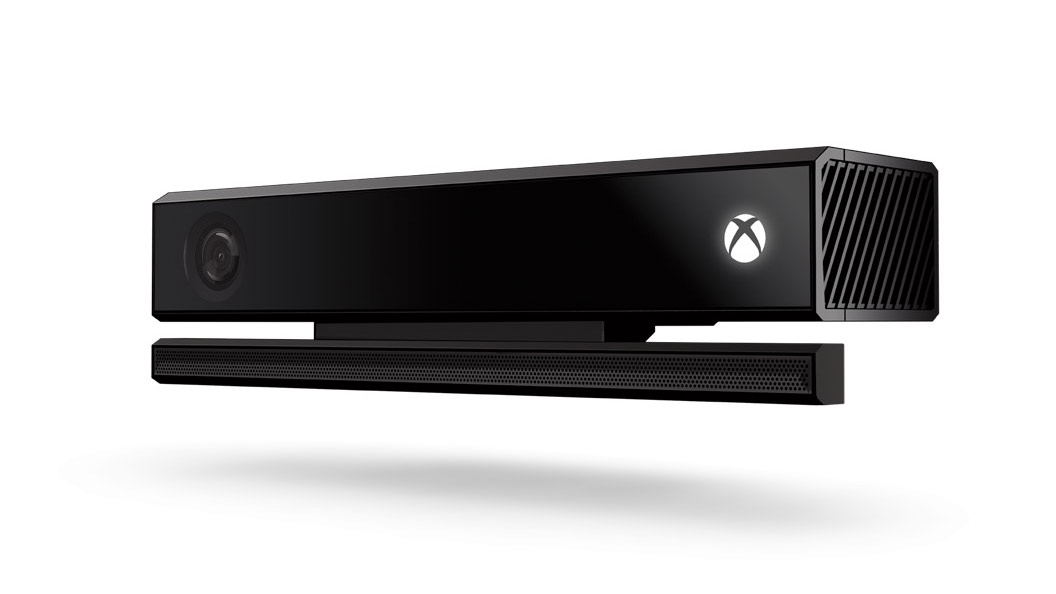
\includegraphics[draft=false, width=5cm]{images/03-foundation/kinect}
	\caption{Microsoft Kinect\textsuperscript{\textregistered} for Xbox ONE.}
	\label{kinect} 
\end{figure}

\begin{table}[H]
\begin{center}
	\begin{tabular}{|c|c|}
		\hline
		sensor dimensions & 24.9 cm $\times$ 6.6 cm $\times$ 6.7 cm\\
		\hline
		sensor weight & approximately 3.1 lbs (1.4 kg) \\
		\hline
		sensor FOV & 70\textsuperscript{$\circ$} x 60\textsuperscript{$\circ$} \\
		\hline
		depth sensing resolution & 512 x 424 \\
		\hline
		max - min depth & 4.5m - 0.4m \\ 
		\hline
		working frequency & 30 hz \\
		\hline 
	\end{tabular}
\end{center}
\caption{Microsof Kinect\textsuperscript{\textregistered} sensor features.}
\label{kinectfeatures}
\end{table}

\subsection{Motors}
The three motors are MAXON 118798 DC motor RE36 GB 70W KL 2WE, whose characteristics are reported in Figure~\ref{motor} and Table~\ref{maxon}.

\begin{figure}[H]
	\centering
	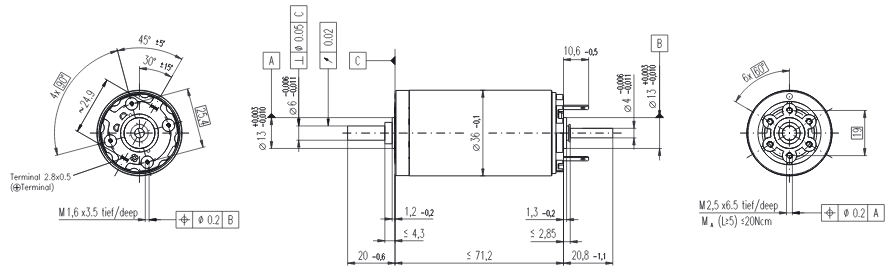
\includegraphics[draft=false, width=\textwidth]{images/03-foundation/motor}
	\caption{MAXON 118798 DC motor schematic. Three units were used in our platform.}
	\label{motor} 
\end{figure}

\begin{table}[h]
	\begin{center}
		\begin{tabular}{|c|c|}
			\hline
			Assigned power rating &  70 W \\
			\hline
			Nominal voltage & 24 V \\
			\hline
			No load speed & 70 x 60  \\
			\hline
			Stall torque & 783 mNm \\
			\hline
			No load current & 105 mA \\ 
			\hline
			Terminal resistance & 1.11 ohm \\
			\hline 
			Max. permissible speed & 8200 rpm \\
			\hline
			Max. efficiency &  85\% \\
			\hline
			Torque constant & 36.4 mNm/A \\
			\hline
			Speed constant & 263 rpm/V \\
			\hline
			Mechanical time constant & 6 ms \\
			\hline 
			Rotor inertia & 67.7 gcm$^2$ \\
			\hline
			Terminal Inductance & 0.2 mH \\
			\hline  
			reduction ratio & [14 : 1] (166158 planetary gear GP32A 2.25NM) \\
			\hline 
		\end{tabular}
	\end{center}
	\caption{MAXON 118798 DC motor parameters.}
    \label{maxon}
\end{table}

\subsubsection{Encoders}
On each motor a 110513 tacho ENCODER HEDS 5540 500IMP 3K is mounted to get the speed of the motor, whose characteristics are reported in Figure~\ref{enc}.
\begin{figure}[htbp]
	\centering
	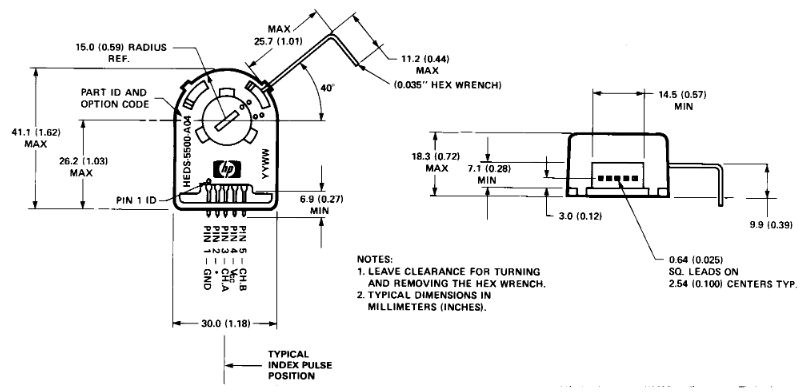
\includegraphics[draft=false,width=\textwidth]{images/03-foundation/enc}
	\caption{Motor encoders deployed for motion sensing and control.}
	\label{enc} 
\end{figure}
E
ncoders contain a single Light Emitting Diode (LED) as its light source. The light is collimated into a parallel beam by means of a single lens located directly over the LED. Opposite the emitter is the integrated detector circuit. This IC consists of multiple sets of photodetectors and the signal processing circuitry necessary to produce the digital waveforms. The code-wheel rotates between the emitter and detector, causing the light beam to be interrupted by the pattern of spaces and bars on the code-wheel. The photodiodes detect these interruptions and send signals to the signal processing circuitry that produces the final outputs that is an index pulse $P_O$ which is generated once for each full rotation of the code-wheel.